% !TEX root = ../paper.tex

\vspace{-5pt}

\section{Evaluation and Discussion}
\label{sec:evaluation}


We implemented \tool by extending \popper with the combined use of
Python ($\sim$200~lines for modifying \popper), \prolog (14 rules for
specificity of predicates, and 19 supported predicates for pure
relations in first-order theories), and ASP ($\sim$200~lines for SL domain knowledge, and $\sim$300~lines for \tool's search space, where 46 rules are used to encode the minimisation rules of the 19 pure relations).
 The prototype of \ggen is implemented by $\sim$50~lines of ASP (to generate the graphs) together with $\sim$100~lines of Python. 
All experiments were conducted on
an 8-core M1 MacBook Pro with 16GB RAM. The valid structure-specific
input memory graphs were either manually/LLM-written, or automatically
generated via \ggen as described in \autoref{sec:generator}.

% As we said in \autoref{sec:normalise}, the entailment of \tool is
% defined by ASP predicate, which might be incomplete. We find it
% effective in our experiment: considering the length of pure relation
% in SL predicates will not be very long, the entailment is enumerable
% within certain length. Here is how to enumerate when adding a new
% theory: if a synthesised predicate is found to be equivalent to a
% shorter one, the theory writer can simply add the corresponding
% entailment relation by an ASP constraint, and repeat until no
% redundancy appears.

% We first discuss the performance of \tool and relevant statistics, then its practical
% utility for program verification and synthesis; we outline its failure modes and possible future work in the end.

% \vspace{-5pt}


\subsection{Benchmarking Predicate Synthesis}
\label{sec:done}

To assess \tool's efficacy as a tool for heap predicate synthesis, our
evaluation addresses the following research questions:
%
\begin{enumerate}[label=\textbf{RQ 1.\arabic*},topsep=2pt,leftmargin=40pt]
\item\label{rq11} \emph{How effective is \tool in synthesising heap predicates?}
\item\label{rq12} \emph{What factors affect the synthesis efficiency?}
\item\label{rq13} \emph{How scalable is \tool with respect to the input size?}
\end{enumerate}




\subsubsection*{\ref{rq11}: Effectiveness and Expressiveness} 
%
We have assembled a set of benchmark for common and
complex heap-based data structures. \autoref{tab:predicates}
summarises our (mostly)\footnote{We will elaborate on the
  partially-successful binomial heap instance~\#15 in
  \autoref{sec:fail}.} successful case studies: 19~Separation~Logic predicates synthesised by \tool within the imposed 20~min
 time limit, which shows that \tool can effectively
produce SL predicates for a variety of heap-based data structures.

In our evaluation, we restricted the predicates in the search space to
feature at \emph{most one pure} theory, since for most predicates, the pure
relations on variables do not influence each other's validity. For
example, the \emph{AVL tree} predicate should feature (1)~a relation
between the heights of a node's subtrees and (2)~ordering relations on
the node payload; any one of these can be encoded independently,
leading to separate SL predicate definitions: \pcode{balanced(A, B)}
for \emph{balanced tree} and \pcode{bst(A, B)} for \emph{binary search
  tree}.
% 
One can then \emph{merge} those two SL predicates with identical
spatial components into a united \emph{AVL tree} \pcode{avl(A, B, C)}
as follows:
%
\begin{enumerate}[topsep=2pt]
\item Merge the parameter lists by appending the pure variables;
\item Merge pure relations  with the overlapped variable renaming;
\item Adapt the recursion in the spatial parts for the new parameter.
\end{enumerate}


\begin{table}[t]
    
  \caption{Statistics on synthesised predicates and the comparison
    with other tool/setting. Columns following the predicate names are
    split by (1) the properties of the predicates: whether a predicate
    is invented (\ie, nested data structure, \underline{PI}), used
    pure relations \underline{Pure}, the size of the output predicate
    \underline{Size} (a triple of arity, the maximal number of
    literals, the maximal number of variables in the predicate); (2)
    the stats of \tool's synthesis: the percentage of run time taken
    by testing the hypotheses \underline{Test\%}, the synthesis time
    of finding the expected hypothesis \underline{T$_0$}, the
    synthesis time of exhaustive search in \textbf{P}ositive-only
    learning \underline{T$_\text{P}$}, 
    %
    (3) the time \underline{T$_\text{I}$} it took to synthesise a
    result when using \popper as the classic \textbf{I}LP to
    synthesise, the time \underline{T$_\text{Io}$} when using classic
    \textbf{I}LP together with our \textbf{o}ptimisation to
    synthesise, and the time \underline{T$_\text{Pd}$} of running
    \textbf{P}OL with SL-based optimisations \textbf{d}isabled
    optimisations; finally, (4) we report the runtimes
    \underline{T$_\text{S}$} of \shape on the same tasks (but without pure relations). All times
    are in seconds, with TO for time-out, ERR for crashes, WA for wrong answers, and NA for not 
    supported in principle.}
\label{tab:predicates}
%    \setlength{\abovecaptionskip}{5pt}
    \centering
    \begin{adjustbox}{width=0.98\textwidth} 
      
      % \footnotesize
      % \begin{adjustbox}{width=0.5\textwidth} 

        \begin{tabular}{cl@{\ }|ccc@{\ }|@{\ }ccc|ccc|c}
          \toprule
          \textbf{No.} &\textbf{Predicate}& \textbf{PI} & \textbf{Pure} & \textbf{Size} & \textbf{Test\%} & \textbf{T$_0$}  & \textbf{T$_\text{P}$} &\textbf{T$_\text{I}$} &\textbf{T$_\text{Io}$} &\textbf{T$_\text{Pd}$} & \textbf{T$_\text{S}$}  \\
          \midrule
          1 &\texttt{singly linked list (payload)}& no & set&       (2,8,5)  & 2\% & $<$1 & 1  & 4 & <1 & 3 & \multirow{2}{*}{{{<1}}}  \\
          2 &\texttt{singly linked list (length)}& no & int&        (2,9,5)  & 1\% & 1 & 9  & NA & NA & 4 &   \\
          3 &\texttt{singly linked list segment}& no & set&         (3,8,6)  & 5\% & $<$1 & 1  & TO & 1 & 31 & 1  \\
          4 &\texttt{doubly linked list}& no & set&                 (3,10,6) & 1\% & 2 & 3  & NA & NA & 339 & 1 \\
          5 &\texttt{doubly linked list segment}& no & set&         (5,10,8) & 1\% & 49 & 192 & TO & 10 &  TO & TO \\
          6 &\texttt{sorted singly linked list}& no & set&          (2,9,5)  & 3\% & $<$1 & 1  & NA & NA & 4 & NA \\
          7 &\texttt{sorted doubly linked list}& no & set&          (3,11,6) & 2\% & 1 & 3  & NA & NA & 231 & NA \\
          8 &\texttt{circular list}& no & set&                      (3,8,6)  & 23\% & $<$1 & 1  & 18 & <1 & 81 & <1  \\
          9 &\texttt{lasso list}& no & set&                         (3,8,6)  & 25\% & $<$1 & 1  & TO & 1 & TO & NA \\
          10 &\texttt{binary tree}&  no & set&                       (2,11,8) & 8\% & 2 &13 & TO & 2 & 245 & WA \\
          11 &\texttt{back-linked tree}&  no & set&                  (3,13,9) & 9\% & 33 & 176 & TO & 41 & TO & TO   \\
          12 &\texttt{binary search tree (set)}& no & set&                 (2,13,8) & 15\% & 11 &26 & NA & NA & TO & \multirow{2}{*}{{{NA}}} \\
          13 &\texttt{binary search tree (list)}& no & list&                (2,13,8) & 39\% & 33 &433  & NA & NA & TO  \\
          14 &\texttt{balanced tree}& no & int&                        (2,12,7) & 32\% & 34 & 458  & NA & NA & TO & NA \\
          15 &\texttt{binomial heap (order)}& no  & int&             (3,14,8) & 33\% & 37 & 1,087  & NA &NA & TO & NA \\
          16 &\texttt{binomial heap (payload)}& no & set&            (3,14,9) & 2\% & 59 & 101  & NA & NA & TO & NA \\
          17 &\texttt{list of lists (set)}& yes & set&                     (2,17,5) & 1\% & 9 &321  & TO & 33 & TO & \multirow{2}{*}{{{ERR}}} \\
          18 &\texttt{list of lists (list)}& yes & list&                      (2,17,5) & 1\%  &14 &759 & TO & 47 & TO  \\
          19 &\texttt{rose (n-ary) tree}& yes & set&                 (2,17,6) & 1\% &9 &749 & NA & NA & TO & ERR \\
          \bottomrule
          \end{tabular}%

  \end{adjustbox}
% {\scriptsize{
    
% }}
%
\end{table}


To show that our positive-only learning (in \autoref{sec:positive})
and the SL-based optimisations (in \autoref{sec:semantics}) are
effective, we compared the synthesis time of \tool with the
unoptimised classic ILP system \popper, \popper with the SL-based
optimisations, and \tool without the optimisations (from left to
right in the table).
%
The results show that (1)~our positive-only learning effectively
learns the predicates which classic ILP cannot discover, and (2)~our
optimisations help to reduce the synthesis time significantly for both
classic ILP and POL for most cases. 
%
The only exception is \#2, where the unoptimised \tool is faster, is
due to the small size of the predicate, where the cost of adding
constraints for reducing the search space is larger than the benefit
of the pruning.
%
%\autoref{sec:fail} discusses the failure scenarios.

We attempted to compare synthesis capabilities of \tool to those
of \shape~\cite{LPAR23:Learning_Data_Structure_Shapes}, the most closely
related work.
%
Like \tool, \shape synthesises SL predicates for data structures from
memory graphs, allowing for positive-only synthesis without negative
examples via meta-interpretive learning
(MIL)~\cite{muggleton2014meta}.
%
However, unlike \tool, \shape only allows one to synthesise a structure's shape
constraints, without any restriction on the data payload or other pure constraints--this is why three data structures (SLL, BST, and a list of lists) with different pure relations are joined in \autoref{tab:predicates} into one predicate per structure in the \shape column \textbf{T$_\text{S}$}.
%
It has been shown in the prior work that the MIL-based learning cannot
define a complete search space for general logic
programs~\cite{cropper2015logical}, which indicates that \shape
\emph{cannot be extended}, even in principle, to express arbitrary
data constraints, such as arithmetic ones.
%
That is, theoretically, 9 (those not marked as NA) out of 16 predicates (with the joining taken into the account) in \autoref{tab:predicates} can be synthesised by \shape. However, in
practice, the bugs in \shape's learning loop implementation resulted in either (1)~the search timing out (TO), (2)~\shape terminating with an error (ERR), or (3)~producing overfitted predicates, \eg, 4 clauses instead of 2 for BST (WA).
%
At the end, we were able to only synthesise 4 predicates with \shape.

% unexpected results (\ie, logic programs within weird formats) results that
% fail the assertion for synthesising nested data structures (even in
% their test suite), together with various bugs when experimenting with
% our benchmark (TO or WA in its column), which end up with only 4 basic
% predicates worked.
%
% \shape's fast runtime is also as expected because of its limited
% expressiveness. With those factors, it does not result in an
% interesting comparison.


% \todo{maybe, two examples of synthesised predicates?}


\subsubsection*{\ref{rq12}: Efficiency}
To understand what affects the synthesis efficiency, let us first look
into the case studies with long synthesis times (more than 5 minutes):
\#13 (BST with list payload), \#14 (balanced tree), \#15 (binomial
heap with order), \#18 (list of lists with list payload), and \#19
(rose tree with set payload).
%
All these case studies feature large predicate sizes, together with
either nested data structures or complex pure theory (integers or
lists). As witnessed by the last two columns of
\autoref{tab:predicates}, the time \tool takes to obtain the expected
predicate is less than 1 minute, and most runtime is spent on the
exhaustive search to give the guarantee of local completeness
(\cf~\autoref{thm:completeness}).
%
It is natural for nested data structures to take long time, because
the increment of search space is applied to both the
synthesis of the auxiliary predicate and the whole predicate.

We also wondered about how the used pure theories affect the
synthesis efficiency.
%
To answer that question, we compare two pairs of predicates (\#12 v.
\#13, \#17 v. \#18) using the same input memory graphs but different
pure theories: sets v. lists. The former is more efficient: this is
because the list is more expressive than set (\eg, a set union with
itself is eliminated, but appending a list to itself is producing a
new list), so the search space is larger after the redundancy
elimination. The same for integer theories: different
combinations of integer operations lead to large search space.

\subsubsection*{\ref{rq13}: Input and Scalability}
Our experiments demonstrate that 2-3 example graphs with tens of nodes
in total (less than 20 node per case study on average in our benchmark
suite) are sufficient to synthesise good predicates (we manually
assessed the results' quality).
%
We report the
fraction of time it took to test the hypotheses during the search.
%
% As for any symbolic machine learning method, the test time of ILP
% system does matter in many learning domains where large number of
% examples are provided as input.
%
In our case, it is not negligible for the examples with complex pure
relations (\eg, \#13-15).
%
In theory the test time should grow \emph{slower than linearly} with
the size of inputs. This is because only correct candidates require
traversing all nodes by the \prolog unification. Since most candidate
predicates do not satisfy all the examples, the testing is terminated
when \prolog reaches the node that falsifies the example.

\begin{figure}[!t]
  \centering  
  \begin{minipage}[t]{0.02\textwidth}
      \centering
      \begin{adjustbox}{width=0.8\textwidth}
        \rotatebox{90}{\small{\qquad\qquad\qquad Testing time (sec)}}
      \end{adjustbox}
  \end{minipage}
  \begin{minipage}[t]{0.45\textwidth}
      \centering
      \begin{adjustbox}{width=0.8\textwidth} 
      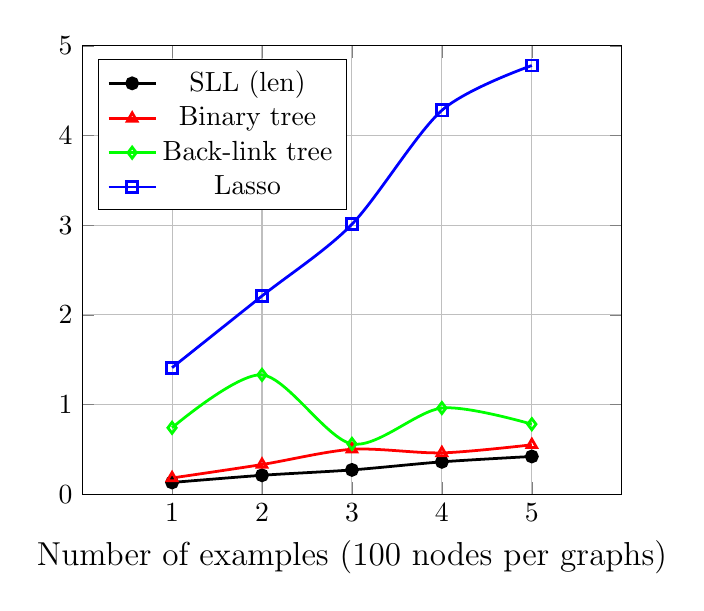
\begin{tikzpicture}
        \begin{axis}[
          xlabel={\large{Number of examples (100 nodes per graphs)}},
          % ylabel={Testing time/sec},
          grid=major,
          xmin=0, xmax=6,
          ymin=0, ymax=5,
          xtick={1,2,3,4,5},
          ytick={0,1,2,3,4,5},
          legend pos=north west,
          ]
          
          \addplot[line width=1pt, smooth, mark=*] coordinates {
            (1, 0.13)
            (2, 0.21)
            (3, 0.27)
            (4, 0.36)
            (5, 0.42)
          };
          
          \addplot[line width=1pt, smooth, mark=triangle, color=red] coordinates {
            (1, 0.18)
            (2, 0.33)
            (3, 0.50)
            (4, 0.46)
            (5, 0.55)
          };
    
          \addplot[line width=1pt, smooth, mark=diamond, color=green] coordinates {
            (1, 0.74)
            (2, 1.33)
            (3, 0.56)
            (4, 0.96)
            (5, 0.78)
          };
          
          \addplot[line width=1pt, smooth, mark=square, color=blue] coordinates {
            (1, 1.41)
            (2, 2.21)
            (3, 3.01)
            (4, 4.28)
            (5, 4.78)
          };
    
          \legend{SLL (len), Binary tree, Back-link tree, Lasso }
        \end{axis}
      \end{tikzpicture}
    \end{adjustbox}
  \end{minipage}
  \begin{minipage}[t]{0.44\textwidth}
    \centering
    \begin{adjustbox}{width=0.8\textwidth}
      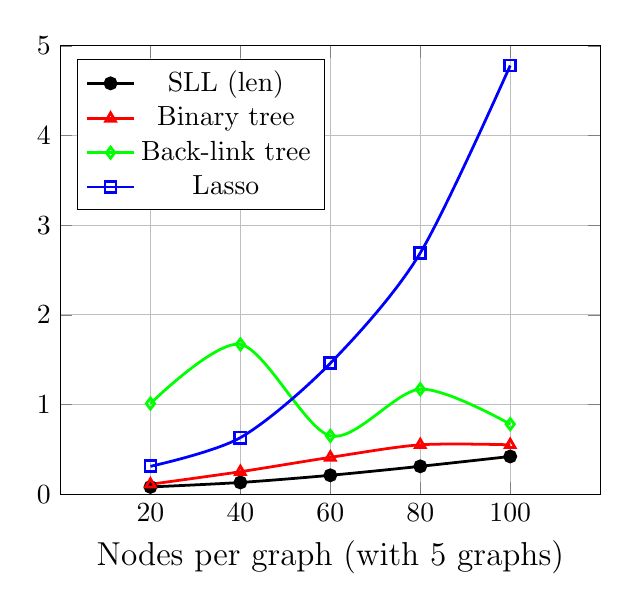
\begin{tikzpicture}
        \begin{axis}[
          xlabel={\large{Nodes per graph (with 5 graphs)}},
          % ylabel={Testing time/sec},
          grid=major,
          xmin=0, xmax=120,
          ymin=0, ymax=5,
          xtick={20,40,60,80,100},
          ytick={0,1,2,3,4,5},
          legend pos=north west,
          ]
          
          \addplot[line width=1pt, smooth, mark=*] coordinates {
            (20, 0.08)
            (40, 0.13)
            (60, 0.21)
            (80, 0.31)
            (100, 0.42)
          };
          
          \addplot[line width=1pt, smooth, mark=triangle, color=red] coordinates {
            (20, 0.11)
            (40, 0.25)
            (60, 0.41)
            (80, 0.55)
            (100, 0.55)
          };
    
          \addplot[line width=1pt, smooth, mark=diamond, color=green] coordinates {
            (20, 1.01)
            (40, 1.67)
            (60, 0.65)
            (80, 1.17)
            (100, 0.78)
          };
          
          \addplot[line width=1pt, smooth, mark=square, color=blue] coordinates {
            (20, 0.31)
            (40, 0.63)
            (60, 1.46)
            (80, 2.69)
            (100, 4.78)
          };
    
          \legend{SLL (len), Binary tree, Back-link tree, Lasso }
        \end{axis}
      \end{tikzpicture}
    \end{adjustbox}    
\end{minipage}
  % \belowcaptionskip=-2pt
%  \abovecaptionskip=3pt
\caption{Testing time  with different input graphs (left); and with different number
    of nodes per graph (right).}
    \label{fig:trend}
\end{figure}


To show scalability of the tool \wrt the input size, 
\autoref{fig:trend} shows the testing time by graph number with
100~nodes per graph on its left, and the testing time by
node number with 5~graphs on its right. The general trends are as expected: the testing time
grows slower than linear in the graph number, and grows linearly in the node number (the percentage of nodes traversed in the examples should be constant with
the same topology of the graph, thus linear). 

Below we discuss the outliers. 
%
The reader can notice the substantial difference between
the testing time of the lasso list case study and every other example.
%
The reason for that is our current implementation of the linearity
check, which is not optimised for \emph{circular} data structures. 
%
Note that the testing of SL predicates consists of two parts: the
 \prolog validity check and the linearity check (in
\autoref{sec:sldomain}), we find that the all but circular data
structures' linearity checking time is negligible. This inefficiency
also explains the faster-than-linear growth of testing times in
\autoref{fig:trend}, and should be solvable by integrating the
checking into \prolog's SLD
resolution~\cite{DBLP:conf/ifip/Kowalski74} (left as
future work).
%
Finally, the testing time of back tree is not even strictly
increasing. The reason is: providing more or larger
examples makes it possible to prune
earlier, thereby reducing the overall synthesis time.
%
% For example, the back tree
% example with 5$*$100 nodes is synthesised in 77s, which is much faster
% than in our basic benchmark (176s).


% It is almost
% consistent with our experiments with both \emph{graph size} and
% \emph{example numbers} changed.
% %
% Notable outliers are the \emph{circular} data structures (\#8 and~9):
% due to the mechanism of \prolog unification, whose graph size has
% significant impact on testing times that degrade worse than linearly.
% \autoref{fig:trend} provides the detailed statistics and discussion
% on these trends.
%

% \vspace{-5pt}

\subsection{The Utility of \tool}
\label{sec:utility}

\subsubsection{Verification}
\label{sec:verification}

Let us demonstrate how the combination of \tool and \ggen facilitates
deductive program verification in SL-based provers. 
%
Specifically, our goal is to streamline the task of writing inductive
predicates, by instead generating them automatically from programs to
be verified.
%
We are interested in the following research questions \wrt the
effectiveness of the approach:

\begin{enumerate}[label=\textbf{RQ 2.\arabic*},topsep=2pt,leftmargin=40pt]
\item\label{rq21} \emph{How much human effort is required to infer the
    predicates?}
  \item\label{rq22} \emph{How effective is \ggen for producing
      positive examples?}
  \item\label{rq23} \emph{Are the inferred predicates the same as the expected
      (human-written) ones, so they can be used directly for the
      verification?}
  \end{enumerate}

  \begin{table}[t]
    \centering
    \caption{Statistics on generating input memory graphs for different
      predicates: the lines of codes of the \code{assert}-annotated
      function or its test, the number of graph instances
      (capped by 100) generated in 10 minutes, the number of asserted
      conjuncts, 
      the ratio of the number of valid graphs to all randomly
      generated graphs, and whether the original program is verified
      with the synthesised predicates against its original
      specification. 
      % 
      For \veri and \grass, \textbf{Y} means verified; we did not manage
      to compile \vcdryad, so \textbf{=} means equivalent to the
      expected predicate, and \textbf{?} means not equivalent and
      couldn't be checked.
  %
  % \todo{Rearrange columns: put Num right before Ratio, add a column for
  %   extra text LOC. I don't understand what is the purpose of mentioning
  % grayed programs if you require tests.}
    }
    \label{tab:gen}
    % \begin{adjustbox} {width=0.48\textwidth}
  {\small{
      \begin{tabular}{l|c|ccccc|c}
        \toprule
        Predicate &Programs &  LOC$_\text{prog}$ & LOC$_\text{test}$ & Assert & Num &Ratio & Verified?\\
        \midrule
        \multirow{2}{*}{{{Singly Linked List}}} & concat\textsuperscript{2} &  10& - & 0& 100 &100\%  & \textbf{Y} \\
        &reverse\textsuperscript{2} &  10& - & 0& 100 &100\%  & \textbf{Y} \\
        \midrule
        \multirow{4}{*}{{{Sorted List}}} & find\textsuperscript{1} &  10& - & 1& 100 &14.4\% & \textbf{=} \\
        &insert\_iter\textsuperscript{1} &  28& - & 2 & 100 &13.3\% & \textbf{=} \\
        &copy\textsuperscript{2} &  26& - & 2 & 100 &13\% & \textbf{Y} \\
        &double\_all\textsuperscript{2} &  25& - & 2 & 100 &12.1\% & \textbf{Y} \\
        \midrule
        \multirow{4}{*}{{{Doubly Linked List}}} &append\textsuperscript{1} &  11& - & 2 &47 & 2.9\% &  \textbf{=} \\
        &dispose\textsuperscript{2} &  9& - & 2 &41 & 2.5\% & \textbf{Y} \\
        &reverse\textsuperscript{3} &  16& - & 2 &47 & 2.9\% & \textbf{Y} \\
        &\graybox{insert\_front\textsuperscript{1}} &  - &10&  2 &47 & 2.9\% & \textbf{=} \\
        \midrule
        % {Circular list} &{N.A.} & \multicolumn{4}{|c}{N.A.} & \textbf{Y} \\
        % \midrule
        \multirow{4}{*}{{{Binary Search Tree}}} & find\textsuperscript{1}  & 16& - & 3& 100 & 11.5\% & \textbf{=} \\
        &insert\textsuperscript{1} &  22& - & 6 &100 & 8.0\% & \textbf{=} \\
        &free\textsuperscript{3} &  11& - & 3 &100 & 7.5\% & \textbf{Y} \\
        &remove\textsuperscript{3} &  43& - & 3 &100 & 12.3\% & \textbf{Y} \\
        \midrule
        \multirow{2}{*}{{{Binomial Heap (order)}}} &\graybox{find\_min\textsuperscript{1}} &  \multirow{2}{*}{- }& \multirow{2}{*}{26} &\multirow{2}{*}{5} &\multirow{2}{*}{18} & \multirow{2}{*}{1.1\%} & \multirow{2}{*}{\textbf{?}} \\
        &\graybox{merge\textsuperscript{1}} &  & &  &  & &  \\
        \bottomrule
              \multicolumn{8}{l}{}
        \\[-8pt]
        \multicolumn{8}{l}{{\textsuperscript{1} From~\vcdryad~\cite{vcdryad}\quad \quad \quad
        \textsuperscript{2} From~\grass~\cite{Piskac-al:TACAS14}\quad \quad \quad
        \textsuperscript{3} From~\veri~\cite{Jacobs-al:NFM11}}}
      \end{tabular}
  }}
    % \end{adjustbox}
  \end{table}
\subsubsection*{\ref{rq21}: Required Human Effort}


For this experiment, we adopted the case studies from benchmark suites
of three different deductive
verifiers~\cite{vcdryad,Piskac-al:TACAS14,Jacobs-al:NFM11}, containing
heap-manipulating programs for different linked data structures, many
of which come with non-trivial data constraints.
%
Our aim is (1)~to quantify the human effort for annotating selected
program(s) with assertions as oracles for graph generation, and (2)~to
confirm that \ggen can produce good-quality graphs for \tool to
synthesise the expected predicates within a reasonable time limit (10
min). For simplicity, we only consider the graphs without cycles
unless being specified (doubly linked list in our case study).




\autoref{tab:gen} shows the statistics for generating up to 100 valid
graphs, with up to five nodes, within the time limit of 10 minutes, to
infer data structure predicates.
%
In all cases, between 0 and~5 simple assertions (\ie, one single
comparison for most cases, except for BST, one of whose assertions is
expressed by a comparison function) are enough for capturing the properties
(\eg, line 7 in \autoref{fig:srtl}).



%
\subsubsection*{\ref{rq22}: Effectiveness of the Graph Generator}

As shown in the table, in each experiment \ggen produced at least 18
valid graphs, which is sufficient for \tool to infer the expected
predicates. Unsurprisingly, the throughput of the generator (\ie,
the Num column in \autoref{tab:gen}) correlates with the
complexity of the predicates: \eg, the binomial heap
instance needs to satisfy not only the order relation between the
nodes but also the heap property, which results in low chances
for the generator to produce valid instances; generally, the throughput is similar (ranged by randomness)
 across programs manipulating the same structure.
%
As expected, the fraction of valid graphs \wrt all randomly generated
can be very low for complex predicates, which shows the importance of
positive-only learning, as large numbers of trivially invalid graphs
would slow down the synthesiser.

% \todo{I don't understand the English text below. Please, use an
%   example: figure, code snippet, etc, and then explain an issue with
%   it. If some programs requres extra test, reflect that in the table
%   in a separate column, showing both LOC of the program and the test,
%   and ignoring the assertions. Furthermore, I don't understand the use
% case for programs like merge then---did you use them for anything?}
%
Even though in principle \ggen could be used for any programs,
%
we found that writing assertions for certain functions
(\graybox{greyboxed} in \autoref{tab:gen}) is not an effective way to
generate the valid instances. 
%
This is because the annotated node might simply not traverse ``enough''
of the structure to perform the validation.
%
As an example, consider inserting a node to the
front of a doubly linked list:
%
\begin{minted}[fontsize=\footnotesize,linenos,numbersep=-10pt]{c}
    DLNode * insert_front(DLNode * x, int k) {
      if (x == NULL) {
        DLNode * head = (DLNode *) malloc(sizeof(DLNode));
        head->key = k;
        head->next = NULL;
        head->prev = NULL;
        return head;
      } else {
        if(x->next != NULL) assert(x->next->prev == x);
        DLNode * head = (DLNode *) malloc(sizeof(DLNode));
        head->key = k;
        head->next = x;
        x->prev = head;
        return head; 
      } 
    }
\end{minted}
%
Testing the following incorrect example of a DLL heap graph, produced
by \ggen, will not violate the assertion at line~9 of the code above.
%
\begin{minted}[fontsize=\small]{prolog}
  next(n1,n2).   next(n2,n3). next(n3,null).
  prev(n1,null). prev(n2,n1). prev(n3,null).
\end{minted}
%
The reason is: the assertion at line~9 is only checked for node
\pcode{n1}, but the offending node \pcode{n2} is not checked because
the function does not traverse the whole list.
%
As a solution, 
%
in cases when no functions manipulating with the structure traverse
the whole structure graph (so their LOCs are not informative, hence
``-'' in \autoref{tab:gen}), one can instead write a standalone
\emph{traversal function} to be used as an oracle. Sizes of those
additional functions are shown as \text{LOC$_\text{test}$} in
\autoref{tab:gen}.
%
% We call them improper because the human effort is more than
% just writing assertions.

We conclude that \ggen is a useful front-end to \tool, but its
effectiveness depends on the ``thoroughness'' of the structure
traversal done by the function that is used as an oracle.



\begin{figure}[b]
  \begin{minted}[fontsize=\footnotesize,linenos,numbersep=-10pt]{c}
      int sorted_find(SNnode * l, int k){
        if (l == NULL) {
          return -1;
        } else if (l->key == k) {
          return 1;
        } else {
          if (l->next != NULL) assert(l->key <= l->next->key);
          int res = sorted_find(l->next, k);
          return res;
        } }
  \end{minted}
  
  \vspace{5pt}  
  
  \begin{minted}[fontsize=\small]{c}
  define pred sorted^(a): 
   ((a l= nil) & emp) | 
   ((a |-> loc next: c; int key: e) * sorted^(c) & (e lt-set keys^(c)))
  \end{minted}
  %\abovecaptionskip=5pt
  % \belowcaptionskip=-5pt
  \caption{An example of the input program with assertions and
    inferred predicate for sorted list in \vcdryad.}
    \label{fig:srtl}
    \end{figure}

\subsubsection*{\ref{rq23}: Quality of Inferred Predicates}



With memory graphs obtained automatically, we synthesised the
respective predicates with \tool and translated them into the syntax
of the corresponding SL-based verifiers (automatically or manually,
based on how complex the concrete verifier's language is).
%
Next, we verified the original programs with the inferred predicates,
thus, demonstrating that the inferred predicates are equivalent to the
expected ones.
%
An inferred sorted list predicate of \vcdryad, corresponding to the
example from \autoref{sec:popper}, is shown in \autoref{fig:srtl}. The
only failing case is the binomial heap with order constraints because
of the limitation of pre-defined predicates in \tool (further
explained in \autoref{sec:fail}), where the synthesised predicates are
partially correct but not strong enough, and need to be refined by
manually adding the missing constraints.



To summarise, we found the combination of \ggen/\tool effective for
automatically producing SL predicates equivalent to human-written ones
from either modestly-annotated programs to be verified, or with a help
of a simple human-written traversal procedure for the data structure.

% the experience to infer SL predicates from given programs
% using \tool the users' efforts to write the predicates, and the
% generator is effective to obtain the instances for the predicates.
% 
% Considering the diversity of SL dialects
% \cite{Appel:ESOP11,DBLP:phd/ethos/Tuerk11,Mueller-al:VMCAI16}, we
% believe that \tool together with the two memory graph extractors can be easily customised to synthesise predicates
% for different SL encodings, then improve the usability of existing
% SL-based tools.

  \begin{figure}[!t]
    \centering  
    \begin{minipage}[b]{0.56\textwidth}
        \centering
        {\footnotesize{
        
    \begin{tabular}{c| c|c|c| c}
    \toprule
    No. & Category & Program & Code/Spec & Time    \\	  
    \midrule
    1 & \multirow{4}{*}{{{Deallocate}}} & sll & 5.5x & 0.2s\\
    2 & & bst & 8.0x & 0.2s\\
    3 & & dll\_seg & 2.4x & 0.2s\\
    4 & & {multilist} & 16.0x & 0.3s\\
    \midrule
    5 &  \multirow{3}{*}{{{Copy}}} & lseg & 2.0x & 0.8s\\
    6 & & bst & 3.5x & 3.3s\\
    7 & & balanced tree & 3.0x & 1.9s\\
    \midrule 
    8 & \multirow{2}{*}{{{Size}}} & sll\_len & 2.1x & 0.4s  \\
    9 & & balanced tree & 3.5x & 0.6s  \\
    \midrule 
    10 & \multirow{8}{*}{{{Transform}}} & sll $\rightarrow$ dlseg & 2.5x & 0.4s  \\
    11 & & {srt\_dll $\rightarrow$ sll} & 3.1x & 7.4s  \\
    12 & & {dll $\rightarrow$ bst} & 15.0x & 42.8s  \\
    13 & & {btree $\rightarrow$ bktree} & 13.6x & 11.8s  \\
    14 & & {multilist $\xrightarrow{}$ sll} & 5.0x & 8.8s  \\
    15 & & {btree $\xrightarrow{}$ dll} & 9.6x & 7.1s  \\
    16 & & {bst $\xrightarrow{}$ srtl} & 11.6x & 10.3s  \\
    17 & & {dll $\xrightarrow{}$ srt\_dll} & 7.3x & 9.3s  \\
      \bottomrule
      %
    \end{tabular}
    
    % & btree $\rightarrow$ dll ? & 1.4x & 0.4  \\

        }}
% \setlength{\belowcaptionskip}{15pt}
      \caption{Example programs synthesised by \suslik from SL
        specifications stated using predicates produced by \tool.}
      
      %
      \label{tab:results}
    \end{minipage}
    \hfill
    \begin{minipage}[b]{0.4\textwidth}
      \centering
      
  \begin{minted}[fontsize=\scriptsize]{c}
  // pre:  {f :-> x ** sorted_dll(x, z, s)}
  // post: {f :-> y ** sll(y, s)}
  
  void srt_dll_to_sll (loc f) {
  loc x1 = READ_LOC(f, 0);
  if (x1 == 0)  {
    WRITE_INT(f, 0, 0);
    return;
  } else {
    int vx11 = READ_INT(x1, 0);
    loc nxtx11 = READ_LOC(x1, 1);
    loc z1 = READ_LOC(x1, 2);
    WRITE_LOC(f, 0, nxtx11);
    srt_dll_to_sll(f);
    loc y11 = READ_LOC(f, 0);
    loc y2 = (loc)malloc(2 * sizeof(loc));
    free(x1);
    WRITE_LOC(f, 0, y2);
    WRITE_LOC(y2, 1, y11);
    WRITE_INT(y2, 0, (int)vx11);
    return;
  }}
  \end{minted}
% \setlength{\belowcaptionskip}{15pt}
  \caption{An example \suslik output (\#{11}): a C program for
    converting a sorted DLL to SLL. \texttt{loc}, \texttt{READ\_LOC},
    \etc are macro-definitions around ordinary C types and operations. }
          \label{fig:transform}
  \end{minipage}
  \end{figure}


\subsubsection{Deductive Synthesis}
\label{sec:synthesis}

As another demonstration of \tool's utility, we employed the
synthesised SL predicates to automatically generate
correct-by-construction heap-manipulating programs in~C using a
state-of-the-art deductive
synthesiser~\suslik~\cite{polikarpova2019structuring,WatanabeGPPS21}.
%
The goal of this exercise was to demonstrate that, one can use \tool
together with \suslik to obtain \emph{provably correct}
implementations of structure-specific procedures for copying,
computing their size, and transformation without knowing how to
specify SL predicates, but using heap graphs. Our case study includes
17 synthesis tasks involving the predicates
from~\autoref{tab:predicates}, producing programs \emph{not} featured
in any past works on \suslik.
%
The average code/spec AST size ratio is 4.1, and the average \suslik
synthesis time is 6.2 sec, which shows that \tool produces predicates
that are \emph{immediately suitable} for proof-driven synthesis.
%
\autoref{tab:results} provides the detailed statistics. An example of
the synthesised C program that transforms a sorted DLL into a singly
linked list is given in \autoref{fig:transform}.

Compared to the existing example-based heap-manipulating program
synthesisers, \spt~\cite{singh2012spt} and
\synbad~\cite{DBLP:conf/sas/Roy13}, the joint \tool/\suslik workflow
does not require ``fold/unfold'' functions (as does \spt) or a
template (as needed by \synbad) for the intended programs.

% \begin{table}[!t]
%   % \setlength{\abovecaptionskip}{5pt}
%     \centering  
%     \caption{Example programs synthesised by \suslik from SL
%     specifications stated using \tool's outputs.}
%   \label{tab:results}
%         {\small{
%         
    \begin{tabular}{c| c|c|c| c}
    \toprule
    No. & Category & Program & Code/Spec & Time    \\	  
    \midrule
    1 & \multirow{4}{*}{{{Deallocate}}} & sll & 5.5x & 0.2s\\
    2 & & bst & 8.0x & 0.2s\\
    3 & & dll\_seg & 2.4x & 0.2s\\
    4 & & {multilist} & 16.0x & 0.3s\\
    \midrule
    5 &  \multirow{3}{*}{{{Copy}}} & lseg & 2.0x & 0.8s\\
    6 & & bst & 3.5x & 3.3s\\
    7 & & balanced tree & 3.0x & 1.9s\\
    \midrule 
    8 & \multirow{2}{*}{{{Size}}} & sll\_len & 2.1x & 0.4s  \\
    9 & & balanced tree & 3.5x & 0.6s  \\
    \midrule 
    10 & \multirow{8}{*}{{{Transform}}} & sll $\rightarrow$ dlseg & 2.5x & 0.4s  \\
    11 & & {srt\_dll $\rightarrow$ sll} & 3.1x & 7.4s  \\
    12 & & {dll $\rightarrow$ bst} & 15.0x & 42.8s  \\
    13 & & {btree $\rightarrow$ bktree} & 13.6x & 11.8s  \\
    14 & & {multilist $\xrightarrow{}$ sll} & 5.0x & 8.8s  \\
    15 & & {btree $\xrightarrow{}$ dll} & 9.6x & 7.1s  \\
    16 & & {bst $\xrightarrow{}$ srtl} & 11.6x & 10.3s  \\
    17 & & {dll $\xrightarrow{}$ srt\_dll} & 7.3x & 9.3s  \\
      \bottomrule
      %
    \end{tabular}
    
    % & btree $\rightarrow$ dll ? & 1.4x & 0.4  \\

%         }}
      
%   % \setlength{\abovecaptionskip}{5pt}
%   % \setlength{\belowcaptionskip}{-10pt}
  
%   \end{table}


% \subsubsection{Other Potential Applications}

% Though not directly evaluated in this work, \tool naturally inherits
% the application domain of other shape analysis tools. 
% %
% Program comprehension and programming education can benefit from the
% generated predicates, as they can be used to
% explain~\cite{marron2012abstracting} or visualise the structures and
% their manipulations~\cite{DBLP:conf/iwpc/BoockmannL22}. 

% \vspace{-5pt}

\subsection{Failure Modes and Future Work}
\label{sec:fail}


In its current version, \tool failed to synthesise predicates for
several intricate linked structures. The reasons for the failed tasks fall into one of the following three categories:

\begin{enumerate}[leftmargin=*,topsep=2pt]
\item \tool's default settings cannot fully capture the structure's
  properties. Consider \#15 from \autoref{tab:predicates}: the root
  and leaf nodes of binomial trees have different order relation with
  their siblings, but our search space cannot express this
  distinction, so the synthesised predicate is \emph{the best in this
    setting} (capturing nodes' ordering \wrt their children) but not
  the expected one.

\item Nested data structures with multiple arguments or complex pure
  relations, For example, the needed search space of the \emph{braced list
    segment} predicate~\cite{Reynolds08} is too large to be fully
  explored within our time limits.

\item An instance of a predicate cannot be proven by top-\emph{down
  evaluation}, so that \prolog cannot evaluate them as expected in SL.
%  (\cf the explanation below).
\end{enumerate}

\noindent
%
In the first case, the solution is naturally to allow richer search space: we might either extend the search space with more predicates (\eg, judging a node is root or not), or enabling larger parameters in \autoref{sec:default} to enrich the expressiveness of \tool.
%
This is in line with a common synthesis trade-off between the
expressiveness and the efficiency; we leave it a future work to find general
search space settings to enrich the expressiveness without much loss
of performance.

In the second case, it is possible to optimise the synthesis of nested
predicates using problem-specific knowledge. For instance, we can
assume the inner data structure is not mutually recursive (as it is in
the case of the braced list segment), reducing the search space by
splitting the synthesis of the auxiliary predicate and the whole
predicate. We leave this optimisation to the future work.


To explain the last issue, consider the following \prolog predicate:
%
\begin{minted}[fontsize=\small]{prolog}
  p(X, Y) :- X == Y.
  p(X, Y) :- next(X, Z), p(Z, Y), p(X, Z).
\end{minted}
%
In plain words: if \pcode{X} and \pcode{Y} have the same location,
then \pcode{p(X, Y)} is true; if not, then the \pcode{p(X, Y)} holds
if the both segments \pcode{p(X, Z)} and \pcode{p(Z, Y)} are true,
where \pcode{Z} is the next node of \pcode{X}.
%
This predicate is valid in Separation Logic, but \prolog rejects it,
because of its validity checking algorithm.
%
To understand the difference that causes the rejection, consider the
literal \pcode{p(a, b)}, in the case when \pcode{next(a, b)} is a fact
that holds.
%
In SL, the literal is true, because it is checked in a
\emph{bottom-up} way, \ie, ``whether the predicate is consistent if it is
true''. Therefore, \pcode{p(a, b)} holds because it is consistent with \pcode{next(a, b), p(b, b), p(a, b)}.
%
However, the test of \pcode{p(a, b)} in \prolog is done in a top-down way,
\ie, ``whether there is a variable unification that makes
\pcode{next(a, Z), p(Z, b), p(a, Z)} true'', which triggers a recursive
test on the inner  \pcode{p(a, b)}. It will be interesting to see whether replacing \prolog with the solvers from SL-COMP \cite{DBLP:conf/tacas/SighireanuPRGIR19} can directly solve it without other overhead.
%

\begin{table}[ht]
\centering
 %Methods with `$^{*}$' means directly using ground truth review text in the testing phase, which are not feasible in practice.



\scalebox{0.9}{
\begin{tabular}{lcccc}
\toprule
LLM & Method &  AUC  & ACC & RMSE \\ \midrule
& NCD & 0.8256 & 0.7759 & 0.3926 \\ 
\midrule
\multirow{2}{*}{GPT-3.5-turbo}& NCD-Beh & 0.8422 &  0.7928 & 0.3781 \\
& NCD-Sem & 0.8460 & 0.7963 & 0.3764\\
\midrule
\multirow{2}{*}{GPT-4o-mini} &NCD-Beh &  0.8454 & 0.7963 & 0.3744\\
&NCD-Sem &  0.8491 & 0.7981 & 0.3715 \\
\midrule
\multirow{2}{*}{GLM-4} & NCD-Beh &  0.8432 & 0.7949 & 0.3758\\
&NCD-Sem &  0.8476 & 0.7975 & 0.3749 \\
 
 \midrule
\multirow{2}{*}{Qwen2.5-72B} & NCD-Beh &  0.8407 & 0.7912 & 0.3795\\
&NCD-Sem &  0.8415 & 0.7938 & 0.3772 \\

\midrule
\multirow{2}{*}{Qwen2.5-14B} & NCD-Beh &  0.8379 & 0.7882 & 0.3813\\
&NCD-Sem &  0.8381 & 0.7906 & 0.3794 \\

 
 \midrule
\multirow{2}{*}{Qwen2.5-coder-7B} & NCD-Beh &  0.8342 & 0.7834 & 0.3854\\
&NCD-Sem &  0.8367 & 0.7862 & 0.3825 \\

\bottomrule 
\end{tabular}}
\caption{Different LLMs on Linux dataset.}
\label{tab:llms}
\end{table}

